% Historical pre-audit source. The revised evaluation is in main.tex.
%% SELF-X -- IEEE conference manuscript
%% Built against the IEEE conference template (IEEEtran, conference option).
%%
%% Every measured number in this document comes from results_macros.tex, which is
%% generated by selfx/scripts/make_paper_macros.py directly from the experiment
%% outputs. Do not type a result by hand: re-run the study and rebuild instead.

\documentclass[conference]{IEEEtran}
\IEEEoverridecommandlockouts
\newtheorem{theorem}{Theorem}

\usepackage[OT1]{fontenc}
\usepackage{cite}
\usepackage{amsmath,amssymb,amsfonts}
\usepackage{algorithm}
\usepackage{algpseudocode}
\usepackage{graphicx}
\usepackage{textcomp}
\usepackage{xcolor}
\usepackage{booktabs}
\usepackage{array}
\usepackage{url}
\usepackage[hidelinks]{hyperref}

% Generated by selfx/scripts/make_paper_macros.py -- do not edit by hand.
% Source study generated 2026-11-09T10:23:01.363500+00:00 (mode: live).

\newcommand{\ResSeeds}{5}
\newcommand{\ResSeedList}{1900, 1901, 1902, 1903, 1904}
\newcommand{\ResWindows}{60}
\newcommand{\ResWindowSec}{5}
\newcommand{\ResTauMs}{100}
\newcommand{\ResEpochSec}{30}
\newcommand{\ResRunSec}{300}
\newcommand{\ResSlotsPerRun}{3000}
\newcommand{\ResTotalSlots}{135,000}
\newcommand{\ResConservation}{8.9e-16}
\newcommand{\ResMode}{live}

\newcommand{\ResZeroLat}{96.94}
\newcommand{\ResZeroLatSem}{4.93}
\newcommand{\ResZeroPNinetyFive}{202.00}
\newcommand{\ResZeroTput}{5.98}
\newcommand{\ResZeroLoss}{32.21}
\newcommand{\ResZeroExcess}{24.24}
\newcommand{\ResZeroReward}{-1.607}
\newcommand{\ResZeroRewardSem}{0.102}
\newcommand{\ResZeroQueue}{0.815}
\newcommand{\ResZeroMaxQueue}{2.000}
\newcommand{\ResZeroCtrl}{0.0}
\newcommand{\ResZeroInstalls}{0.0}
\newcommand{\ResZeroVetoes}{0.0}
\newcommand{\ResZeroBound}{0.00}
\newcommand{\ResZeroConv}{300.0}
\newcommand{\ResOneLat}{92.00}
\newcommand{\ResOneLatSem}{4.44}
\newcommand{\ResOnePNinetyFive}{201.15}
\newcommand{\ResOneTput}{6.13}
\newcommand{\ResOneLoss}{30.47}
\newcommand{\ResOneExcess}{22.51}
\newcommand{\ResOneReward}{-1.489}
\newcommand{\ResOneRewardSem}{0.094}
\newcommand{\ResOneQueue}{0.786}
\newcommand{\ResOneMaxQueue}{2.594}
\newcommand{\ResOneCtrl}{3526.0}
\newcommand{\ResOneInstalls}{13.6}
\newcommand{\ResOneVetoes}{14.2}
\newcommand{\ResOneBound}{0.00}
\newcommand{\ResOneConv}{300.0}
\newcommand{\ResTwoLat}{82.22}
\newcommand{\ResTwoLatSem}{5.51}
\newcommand{\ResTwoPNinetyFive}{200.62}
\newcommand{\ResTwoTput}{6.37}
\newcommand{\ResTwoLoss}{27.89}
\newcommand{\ResTwoExcess}{19.92}
\newcommand{\ResTwoReward}{-1.246}
\newcommand{\ResTwoRewardSem}{0.111}
\newcommand{\ResTwoQueue}{0.724}
\newcommand{\ResTwoMaxQueue}{2.470}
\newcommand{\ResTwoCtrl}{4361.8}
\newcommand{\ResTwoInstalls}{20.2}
\newcommand{\ResTwoVetoes}{19.4}
\newcommand{\ResTwoBound}{0.00}
\newcommand{\ResTwoConv}{300.0}
\newcommand{\ResThreeLat}{83.51}
\newcommand{\ResThreeLatSem}{5.75}
\newcommand{\ResThreePNinetyFive}{199.98}
\newcommand{\ResThreeTput}{6.16}
\newcommand{\ResThreeLoss}{30.17}
\newcommand{\ResThreeExcess}{22.20}
\newcommand{\ResThreeReward}{-1.319}
\newcommand{\ResThreeRewardSem}{0.121}
\newcommand{\ResThreeQueue}{0.714}
\newcommand{\ResThreeMaxQueue}{2.366}
\newcommand{\ResThreeCtrl}{397.6}
\newcommand{\ResThreeInstalls}{21.2}
\newcommand{\ResThreeVetoes}{30.6}
\newcommand{\ResThreeBound}{0.00}
\newcommand{\ResThreeConv}{300.0}
\newcommand{\ResFourLat}{84.08}
\newcommand{\ResFourLatSem}{4.64}
\newcommand{\ResFourPNinetyFive}{198.00}
\newcommand{\ResFourTput}{6.41}
\newcommand{\ResFourLoss}{27.42}
\newcommand{\ResFourExcess}{19.45}
\newcommand{\ResFourReward}{-1.276}
\newcommand{\ResFourRewardSem}{0.096}
\newcommand{\ResFourQueue}{0.741}
\newcommand{\ResFourMaxQueue}{2.450}
\newcommand{\ResFourCtrl}{358.9}
\newcommand{\ResFourInstalls}{17.6}
\newcommand{\ResFourVetoes}{9.2}
\newcommand{\ResFourBound}{0.00}
\newcommand{\ResFourConv}{300.0}
\newcommand{\ResFiveLat}{53.92}
\newcommand{\ResFiveLatSem}{3.91}
\newcommand{\ResFivePNinetyFive}{187.43}
\newcommand{\ResFiveTput}{7.02}
\newcommand{\ResFiveLoss}{20.63}
\newcommand{\ResFiveExcess}{12.66}
\newcommand{\ResFiveReward}{-0.549}
\newcommand{\ResFiveRewardSem}{0.082}
\newcommand{\ResFiveQueue}{0.488}
\newcommand{\ResFiveMaxQueue}{3.151}
\newcommand{\ResFiveCtrl}{331.0}
\newcommand{\ResFiveInstalls}{21.2}
\newcommand{\ResFiveVetoes}{580.8}
\newcommand{\ResFiveBound}{0.00}
\newcommand{\ResFiveConv}{300.0}
\newcommand{\ResThrLat}{88.88}
\newcommand{\ResThrLatSem}{4.57}
\newcommand{\ResThrPNinetyFive}{202.00}
\newcommand{\ResThrTput}{6.23}
\newcommand{\ResThrLoss}{29.44}
\newcommand{\ResThrExcess}{21.47}
\newcommand{\ResThrReward}{-1.407}
\newcommand{\ResThrRewardSem}{0.098}
\newcommand{\ResThrQueue}{0.769}
\newcommand{\ResThrMaxQueue}{2.369}
\newcommand{\ResThrCtrl}{0.0}
\newcommand{\ResThrInstalls}{15.6}
\newcommand{\ResThrVetoes}{18.2}
\newcommand{\ResThrBound}{0.00}
\newcommand{\ResThrConv}{300.0}
\newcommand{\ResLstLat}{82.83}
\newcommand{\ResLstLatSem}{5.12}
\newcommand{\ResLstPNinetyFive}{198.63}
\newcommand{\ResLstTput}{6.44}
\newcommand{\ResLstLoss}{27.01}
\newcommand{\ResLstExcess}{19.04}
\newcommand{\ResLstReward}{-1.246}
\newcommand{\ResLstRewardSem}{0.108}
\newcommand{\ResLstQueue}{0.730}
\newcommand{\ResLstMaxQueue}{2.533}
\newcommand{\ResLstCtrl}{0.0}
\newcommand{\ResLstInstalls}{18.4}
\newcommand{\ResLstVetoes}{0.6}
\newcommand{\ResLstBound}{0.00}
\newcommand{\ResLstConv}{300.0}
\newcommand{\ResTabLat}{74.78}
\newcommand{\ResTabLatSem}{6.35}
\newcommand{\ResTabPNinetyFive}{193.75}
\newcommand{\ResTabTput}{6.23}
\newcommand{\ResTabLoss}{29.35}
\newcommand{\ResTabExcess}{21.38}
\newcommand{\ResTabReward}{-1.131}
\newcommand{\ResTabRewardSem}{0.137}
\newcommand{\ResTabQueue}{0.642}
\newcommand{\ResTabMaxQueue}{2.614}
\newcommand{\ResTabCtrl}{0.0}
\newcommand{\ResTabInstalls}{26.2}
\newcommand{\ResTabVetoes}{24.0}
\newcommand{\ResTabBound}{0.00}
\newcommand{\ResTabConv}{300.0}

\newcommand{\ResFloorLoss}{7.97}
\newcommand{\ResLatVsStatic}{44.4}
\newcommand{\ResLossVsStatic}{36.0}
\newcommand{\ResQueueVsStatic}{40.1}
\newcommand{\ResLatVsQ}{27.9}
\newcommand{\ResLossVsQ}{29.7}
\newcommand{\ResLatVsLLM}{41.4}

\newcommand{\ResFastUs}{33.1}
\newcommand{\ResFastPNinetyNineUs}{78.7}
\newcommand{\ResSpeedup}{96,343}
\newcommand{\ResSpeedupChain}{106,457}

\newcommand{\ResLLMModel}{openrouter:nvidia/nemotron-3.5-lightning:free}
\newcommand{\ResLLMChain}{8}
\newcommand{\ResLLMDecisions}{250}
\newcommand{\ResLLMRequests}{90}
\newcommand{\ResLLMCached}{160}
\newcommand{\ResLLMFallbacks}{0}
\newcommand{\ResLLMServed}{100.0}
\newcommand{\ResLLMLatency}{3191}
\newcommand{\ResLLMPNinetyFive}{4956}
\newcommand{\ResLLMChainLatency}{10794}
\newcommand{\ResLLMChainPNinetyFive}{42765}
\newcommand{\ResLLMTripped}{5}
\newcommand{\ResLLMPromptTokens}{79,804}
\newcommand{\ResLLMUniqueModels}{1}
\newcommand{\ResLLMServedBy}{gemini:gemini-3.1-flash-lite}
\newcommand{\ResLLMServedByCount}{250}
\newcommand{\ResLLMServedByPct}{100.0}
\newcommand{\ResLoRAInference}{363}
\newcommand{\ResLoRACalls}{900}

\newcommand{\StatSFivevsSZeroT}{11.661}
\newcommand{\StatSFivevsSZeroP}{$<10^{-12}$}
\newcommand{\StatSFivevsSZeroD}{0.67}
\newcommand{\StatSFivevsSZeroN}{300}
\newcommand{\StatSFivevsSZeroCILo}{0.87}
\newcommand{\StatSFivevsSZeroCIHi}{1.22}
\newcommand{\StatSFivevsSOneT}{10.914}
\newcommand{\StatSFivevsSOneP}{$<10^{-12}$}
\newcommand{\StatSFivevsSOneD}{0.63}
\newcommand{\StatSFivevsSOneN}{300}
\newcommand{\StatSFivevsSOneCILo}{0.80}
\newcommand{\StatSFivevsSOneCIHi}{1.07}
\newcommand{\StatSFivevsSTwoT}{9.751}
\newcommand{\StatSFivevsSTwoP}{$<10^{-12}$}
\newcommand{\StatSFivevsSTwoD}{0.56}
\newcommand{\StatSFivevsSTwoN}{300}
\newcommand{\StatSFivevsSTwoCILo}{0.56}
\newcommand{\StatSFivevsSTwoCIHi}{0.85}
\newcommand{\StatSFivevsSThreeT}{10.052}
\newcommand{\StatSFivevsSThreeP}{$<10^{-12}$}
\newcommand{\StatSFivevsSThreeD}{0.58}
\newcommand{\StatSFivevsSThreeN}{300}
\newcommand{\StatSFivevsSThreeCILo}{0.64}
\newcommand{\StatSFivevsSThreeCIHi}{0.92}
\newcommand{\StatSFivevsSFourT}{9.771}
\newcommand{\StatSFivevsSFourP}{$<10^{-12}$}
\newcommand{\StatSFivevsSFourD}{0.56}
\newcommand{\StatSFivevsSFourN}{300}
\newcommand{\StatSFivevsSFourCILo}{0.62}
\newcommand{\StatSFivevsSFourCIHi}{0.81}
\newcommand{\StatSFivevsQT}{8.880}
\newcommand{\StatSFivevsQP}{$<10^{-12}$}
\newcommand{\StatSFivevsQD}{0.51}
\newcommand{\StatSFivevsQN}{300}
\newcommand{\StatSFivevsQCILo}{0.44}
\newcommand{\StatSFivevsQCIHi}{0.73}
\newcommand{\StatLatSFivevsSZeroT}{-11.723}
\newcommand{\StatLatSFivevsSZeroP}{$<10^{-12}$}
\newcommand{\StatLatSFivevsSZeroD}{-0.68}
\newcommand{\StatLatSFivevsSZeroN}{300}
\newcommand{\StatLatSFivevsSZeroCILo}{-49.84}
\newcommand{\StatLatSFivevsSZeroCIHi}{-34.62}
\newcommand{\StatLossSFivevsSZeroT}{-11.190}
\newcommand{\StatLossSFivevsSZeroP}{$<10^{-12}$}
\newcommand{\StatLossSFivevsSZeroD}{-0.65}
\newcommand{\StatLossSFivevsSZeroN}{300}
\newcommand{\StatLossSFivevsSZeroCILo}{-8.82}
\newcommand{\StatLossSFivevsSZeroCIHi}{-6.19}
\newcommand{\StatBonferroni}{0.0063}

\newcommand{\ResAdapterBase}{0.273}
\newcommand{\ResAdapterCandidate}{0.455}
\newcommand{\ResAdapterGain}{0.182}
\newcommand{\ResAdapterMargin}{0.02}
\newcommand{\ResAdapterDecision}{promoted}
\newcommand{\ResAdapterEpisodes}{150}
\newcommand{\ResAdapterStates}{24}
\newcommand{\ResAdapterTrainStates}{13}
\newcommand{\ResAdapterGateStates}{11}
\newcommand{\ResAdapterParams}{460,800}
\newcommand{\ResAdapterSteps}{60}
\newcommand{\ResAdapterRank}{8}
\newcommand{\ResAdapterAlpha}{16}

\newcommand{\ResVMin}{1.0}
\newcommand{\ResVMax}{32.0}
\newcommand{\ResVBacklogMin}{0.044}
\newcommand{\ResVBacklogMax}{0.112}
\newcommand{\ResVLossMin}{2.11}
\newcommand{\ResVLossMax}{2.06}
\newcommand{\ResVCompliance}{100.0}

\newcommand{\ResTransferProfile}{flash\_crowd}
\newcommand{\ResTransferRetention}{73.0}
\newcommand{\ResTransferTrainGain}{2.014}
\newcommand{\ResTransferHoldGain}{1.470}

% --- Table: staged ablation ---
\newcommand{\AblationRows}{%
S0 & 96.94 & 202.00 & 5.98 & 32.21 & 0.815 & -1.607 \\
S1 & 92.00 & 201.15 & 6.13 & 30.47 & 0.786 & -1.489 \\
S2 & 82.22 & 200.62 & 6.37 & 27.89 & 0.724 & -1.246 \\
S3 & 83.51 & 199.98 & 6.16 & 30.17 & 0.714 & -1.319 \\
S4 & 84.08 & 198.00 & 6.41 & 27.42 & 0.741 & -1.276 \\
\bfseries S5 & \bfseries 53.92 & \bfseries 187.43 & \bfseries 7.02 & \bfseries 20.63 & \bfseries 0.488 & \bfseries -0.549 \\
}

% --- Table: baseline comparison ---
\newcommand{\BaselineRows}{%
Static OpenFlow (no control) & 96.94 & 202.00 & 32.21 & -1.607 & 0.0 \\
Capacity-aware threshold & 88.88 & 202.00 & 29.44 & -1.407 & 0.0 \\
Greedy least-loaded (ECMP-style) & 82.83 & 198.63 & 27.01 & -1.246 & 0.0 \\
Tabular $Q$-learning & 74.78 & 193.75 & 29.35 & -1.131 & 0.0 \\
Zero-shot LLM agent & 92.00 & 201.15 & 30.47 & -1.489 & 3526.0 \\
Reflexive LLM + self-critique & 82.22 & 200.62 & 27.89 & -1.246 & 4361.8 \\
\textbf{SELF-X (proposed)} & \bfseries 53.92 & \bfseries 187.43 & \bfseries 20.63 & \bfseries -0.549 & \bfseries 331.0 \\
}


\newcommand{\dpi}{\Delta\pi}
\newcommand{\Qvec}{\mathbf{Q}}
\newcommand{\wvec}{\mathbf{w}}

\begin{document}

\title{SELF-X: A Three-Timescale Decomposition for Language-Model-Governed\\
Flow Control in Software-Defined Networks}

\author{%
\IEEEauthorblockN{Ganesh Reddy J\IEEEauthorrefmark{1},
M Jagadeswar\IEEEauthorrefmark{1},
Harsh Raj\IEEEauthorrefmark{1},\\
C Sai Aravind\IEEEauthorrefmark{1},
Koushik C\IEEEauthorrefmark{2},
Dhruv R Katti\IEEEauthorrefmark{3}}
\IEEEauthorblockA{%
\IEEEauthorrefmark{1}Dept.\ of Data Science and Artificial Intelligence\\
\IEEEauthorrefmark{2}Dept.\ of Computer Science and Engineering\\
\IEEEauthorrefmark{3}Dept.\ of Electronics and Communication Engineering\\
\textit{Indian Institute of Information Technology Dharwad}, Dharwad, Karnataka, India\\
Team SDN\_07 --- EC466 Software Defined Networks\\
\{23bds024, 23bds033, 23bds076, 23bds075, 23bcs073, 23bec015\}@iiitdwd.ac.in}
}

\maketitle

\begin{abstract}
Language-model agents are an attractive control plane for software-defined
networks because they reason over heterogeneous telemetry without a reward
engineer, but they are far too slow and too unreliable to touch a congested
datapath directly. Existing agentic SDN work either keeps the model in the
decision path and inherits its latency, or bolts a governance layer onto a
learned controller without ever measuring what the governance costs. We argue
that the useful question is not whether a language model can control a network,
but \emph{at which timescale each mechanism earns its place}, and we answer it by
measurement. SELF-X decomposes control into three loops whose periods are set by
the measured cost of the mechanism that runs in them: a Lyapunov
drift-plus-penalty optimiser every \ResTauMs~ms, a weight-internalised LoRA policy
head every \ResWindowSec~s, and a remote multi-agent language-model governor
every \ResEpochSec~s that emits only a safety-gated policy delta
$\dpi=(V,\wvec,\mathcal{M})$ and never an individual flow rule. We evaluate a
six-stage incremental pipeline --- static forwarding, a static LLM agent, $+$
self-critique, $+$ LoRA fine-tuning, $+$ multi-agent governance, $+$ the fast
Lyapunov loop --- on an identical bit-conserving fluid datapath across
\ResSeeds~paired seeds and \ResTotalSlots~control slots, with every language-model
decision served by a live free-tier endpoint and recorded for exact replay. The
full pipeline cuts mean delay by \ResLatVsStatic\% and packet loss by
\ResLossVsStatic\% against static OpenFlow forwarding, and by \ResLatVsLLM\%
against the static LLM agent, while the fast loop decides in \ResFastUs~\textmu s
against a measured \ResLLMLatency~ms for one healthy free-tier model request ---
a factor of roughly \ResSpeedup. We also report what the ablation does \emph{not} show, and we
separate the loss any controller could remove from the \ResFloorLoss\% that is
imposed by offered demand exceeding total capacity.
\end{abstract}

\begin{IEEEkeywords}
Software-defined networking, OpenFlow, Lyapunov optimisation, drift-plus-penalty,
LLM agents, multi-agent systems, LoRA, reproducibility.
\end{IEEEkeywords}

% =====================================================================
\section{Introduction}
% =====================================================================

A software-defined network separates a programmable control plane from the
forwarding hardware beneath it~\cite{mckeown2008openflow}. The traffic that plane
has to manage is bimodal: latency-sensitive \emph{mice} flows share a bottleneck
with bursty, bandwidth-hungry \emph{elephant} flows~\cite{alizadeh2010dctcp}. When
the two collide, shallow switch buffers fill in tens of milliseconds and the mice
pay for it in tail latency and loss.

Three families of controller address this. Static heuristics such as
ECMP~\cite{hopps2000ecmp} are instantaneous and buffer-blind. Deep reinforcement
learners adapt, but need many thousands of interactions before they are useful and
explore unsafely while they learn~\cite{xu2018experience}. Most recently,
language-model agents have been proposed as controllers that reason over raw
telemetry without a hand-designed reward~\cite{araujo2024agentic,li2026redsi,
jamshidi2026governance}.

The language-model route has an awkward fact at its centre, which the literature
tends to state qualitatively and then move past: a remote model takes on the order
of a second to answer, and a congested 10~Mbps link with a 2~Mbit buffer saturates
in about 200~ms. A controller whose decision arrives after the buffer has already
overflowed is not a controller. Our measurements make the gap concrete: one
healthy free-tier model request in our study costs \ResLLMLatency~ms on average
(95th percentile \ResLLMPNinetyFive~ms), and the slow loop's end-to-end wait per
decision reaches \ResOneCtrl~ms once the walk past endpoints that have exhausted
their daily allowance is counted, while the analytic fast-loop optimiser decides
in \ResFastUs~\textmu s.

That observation reframes the design question. Rather than asking whether a
language model can control a network, we ask \emph{what each mechanism costs to
run, and therefore how often it can be run}. The answer is a three-timescale
decomposition in which every loop period is justified by a measured number rather
than chosen by convention, and in which the language model is confined to the one
job its latency permits: setting the objective, not installing the rules.

\textbf{Contributions.}
\begin{enumerate}
  \item \textbf{A cost-justified three-timescale decomposition.} We place a
    Lyapunov drift-plus-penalty optimiser at \ResTauMs~ms, a weight-internalised
    LoRA policy head at \ResWindowSec~s, and a remote multi-agent governor at
    \ResEpochSec~s, and we show by measurement that each period is the smallest
    that the mechanism's own latency allows (Section~\ref{sec:results-latency}).
  \item \textbf{A strictly incremental six-stage ablation} --- static,
    static LLM, $+$self-critique, $+$LoRA, $+$multi-agent governance, $+$fast
    Lyapunov loop --- where consecutive stages differ by exactly one mechanism and
    all stages see bit-identical offered demand (Section~\ref{sec:results-ablation}).
  \item \textbf{An honest loss accounting.} We compute the loss floor imposed by
    demand exceeding total capacity and report it separately, so that the
    controller is only credited with the loss it could actually have removed
    (Section~\ref{sec:results-loss}).
  \item \textbf{A record-and-replay reproducibility contract.} Every
    language-model request is recorded with its prompt hash, served endpoint,
    latency and token count; a reviewer with no API key reproduces every number in
    this paper byte-for-byte from the recorded trace
    (Section~\ref{sec:reproducibility}).
\end{enumerate}

We also report negative and partial results plainly. The multi-agent governance
stage does not dominate the LoRA stage on every metric, and we say so and explain
why in Section~\ref{sec:discussion}.

% =====================================================================
\section{Related Work and Positioning}\label{sec:related}
% =====================================================================

\textbf{Lyapunov control of queueing networks.} Drift-plus-penalty descends from
the max-weight stability results of Tassiulas and
Ephremides~\cite{tassiulas1992stability} and the general framework of
Neely~\cite{neely2010stochastic}. It gives an $O(V)$ backlog / $O(1/V)$ penalty
trade-off with no model of the arrival process and no training. What it does
\emph{not} give is any way to choose $V$, the penalty weights $\wvec$, or the
admissible action set for a workload nobody has seen before. Those are exactly the
quantities our slow loop sets.

\textbf{Multi-agent RL for SDN traffic control.} Boussaoud \emph{et
al.}~\cite{boussaoud2025marl} detect congestion and steer traffic in an SDN with
data-driven multi-agent reinforcement learning. Their agents learn the control
policy itself, so they inherit the cold-start and unsafe-exploration cost of RL
and give no analytic backlog guarantee. In SELF-X the learned components never
choose a rate or a port directly: the fast loop is analytic and carries the bound,
and learning is confined to the objective parameters above it.

\textbf{Reflexive LLM agents for SDN.} Araujo \emph{et
al.}~\cite{araujo2024agentic} propose a reflexive LLM agent architecture that
perceives network and application data and acts on it, going beyond intent parsing
to execution. This is the closest prior work to our stage S1--S2, and we implement
it as an explicit comparison rather than describing it: our static LLM agent and
our self-critique stage are instantiations of that design on our datapath. Our
finding is that the reflexive design helps (Table~\ref{tab:ablation}) but is
bounded by its own request latency, which no amount of better prompting removes.

\textbf{Reflection distilled into weights.} Li \emph{et al.}~\cite{li2026redsi}
argue that prompt-resident reflection loses long-horizon history to the context
window, and distil interaction experience into a small language model's parameters
through preference-based fine-tuning for RAN slicing. We adopt the same conclusion
for a different reason: in our setting the decisive advantage of moving experience
into weights is not context length but \emph{latency}. A local LoRA-adapted
135M-parameter head answers in \ResThreeCtrl~ms against \ResLLMLatency~ms for one
remote request, which is what lets the policy run once per \ResWindowSec~s window
instead of once per \ResEpochSec~s epoch. Reflexion~\cite{shinn2023reflexion} and
LoRA~\cite{hu2022lora} supply the verbal-feedback and low-rank-adaptation
machinery we build on.

\textbf{LLM governance over a two-timescale learner.} Jamshidi \emph{et
al.}~\cite{jamshidi2026governance} are the nearest neighbour to this work: per-switch
PPO agents act on a fast timescale under action masking, while a multi-agent LLM
governance engine proposes machine-parsable $\Delta\Pi$ updates to a policy
constitution, admitted only after non-regression and safety stress tests. We share
the $\dpi$ channel, the fail-closed gate and the refusal to let the model emit
rules. Three things differ. First, their fast layer is a \emph{learned} PPO policy;
ours is an analytic Lyapunov optimiser, so backlog stability is a theorem
(Section~\ref{sec:theory}) rather than an empirical observation, and there is no
cold start. Second, they report a two-timescale split, whereas our measurements
force a \emph{third} timescale between the two: the remote model is too slow even
for the per-window layer, and the LoRA head exists specifically to fill that gap.
Third, and most practically, we treat the governance layer's own cost as a
first-class measured quantity --- request latency, served fraction, declared
fallbacks and free-tier daily request ceilings --- instead of assuming the model is
always available.

\begin{table}[t]
\caption{Positioning against the four closest systems. ``LLM cost priced'' means
the paper reports what consulting the model costs in latency and availability,
rather than assuming it is free.}
\label{tab:positioning}
\centering
\footnotesize
\renewcommand{\arraystretch}{1.18}
\setlength{\tabcolsep}{3.2pt}
\begin{tabular}{lcccc}
\toprule
\textbf{System} & \textbf{Fast layer} & \textbf{Backlog} & \textbf{LLM} & \textbf{LLM cost} \\
 & & \textbf{guarantee} & \textbf{emits} & \textbf{priced} \\
\midrule
Boussaoud \cite{boussaoud2025marl} & MARL        & none      & ---            & n/a \\
Araujo \cite{araujo2024agentic}    & LLM agent   & none      & actions        & no \\
Li \cite{li2026redsi}              & tuned SLM   & none      & actions        & no \\
Jamshidi \cite{jamshidi2026governance} & PPO     & empirical & $\Delta\Pi$    & no \\
\textbf{SELF-X} & \textbf{analytic DPP} & \textbf{theorem} & \textbf{$\dpi$ only}
  & \textbf{yes} \\
\bottomrule
\end{tabular}
\end{table}

\textbf{Summary of the gap.} Across these four works, the fast layer is either
unguaranteed (learned) or unadaptive (fixed heuristic); the language model is
either in the decision path or priced at zero; and the ablation that would separate
the contributions --- static agent, $+$self-critique, $+$weight adaptation, $+$
multi-agent governance, $+$fast analytic loop --- is not run end-to-end on one
datapath. That ablation is the core of this paper.

% =====================================================================
\section{Problem Scenario and System Model}\label{sec:model}
% =====================================================================

\subsection{Scenario}
A linear four-switch OpenFlow~1.3 topology carries traffic between an ingress and
an egress switch over two parallel logical paths: a short \emph{primary} path and a
longer \emph{alternate} trunk. A steady mice aggregate $m(t)$ must stay on the
primary path, because it is the low-propagation route and the traffic is
latency-sensitive. A bursty elephant aggregate $e(t)$ is the only traffic the
controller may move or meter. Table~\ref{tab:params} lists every constant.

\begin{table}[t]
\caption{Model and experiment constants, fixed before any run}
\label{tab:params}
\centering
\renewcommand{\arraystretch}{1.12}
\begin{tabular}{llr}
\toprule
\textbf{Symbol} & \textbf{Meaning} & \textbf{Value} \\
\midrule
$C_0, C_1$      & path capacity (primary, alternate) & 10 Mbps \\
$B_{\text{buf}}$& per-path buffer                    & 2.0 Mbit \\
$D_0, D_1$      & propagation delay                  & 2, 12 ms \\
$\tau$          & fast control slot                  & \ResTauMs\ ms \\
$T_w$           & control window                     & \ResWindowSec\ s \\
$T_g$           & governance epoch                   & \ResEpochSec\ s \\
$V$             & Lyapunov penalty weight (initial)  & 8.0 \\
$\varepsilon$   & capacity-region slack              & 0.6 \\
--              & safety drop ceiling / meter floor  & 20\%, 512 kbps \\
--              & seeds $\times$ windows per run     & \ResSeeds\ $\times$ \ResWindows \\
\bottomrule
\end{tabular}
\end{table}

\subsection{Datapath dynamics}
Time is slotted at $\tau$. Writing $\lambda_i(t)$ for the arrival rate steered onto
path $i\in\{0,1\}$ and $Q_i(t)$ for its backlog in Mbit, one slot evolves as
\begin{align}
\tilde{Q}_i(t)   &= Q_i(t) + (\lambda_i(t) - C_i)\,\tau, \label{eq:raw}\\
Q_i(t{+}1)       &= \min\!\big(B_{\text{buf}},\,\max(0,\tilde{Q}_i(t))\big), \label{eq:clip}\\
o_i(t)           &= \max\!\big(0,\ \tilde{Q}_i(t) - B_{\text{buf}}\big), \label{eq:overflow}\\
s_i(t)           &= Q_i(t) + \lambda_i(t)\tau - Q_i(t{+}1) - o_i(t), \label{eq:served}
\end{align}
where $o_i$ is tail-drop overflow and $s_i$ is bits served. Equations
\eqref{eq:raw}--\eqref{eq:served} conserve bits exactly,
$Q_i(t)+\lambda_i(t)\tau = s_i(t)+o_i(t)+Q_i(t{+}1)$, and the implementation
asserts this identity on every slot of every run; the largest residual observed
across the whole study is \ResConservation~Mbit, which is floating-point noise.

A \texttt{rate\_limit} action installs an OpenFlow meter admitting
$\min(e(t), r/1000)$ Mbps and metering the remainder away; metered bits are counted
as loss, not hidden. Delay on a path is propagation plus a Little's-law queueing
term,
\begin{equation}
d_i(t) = D_i + 1000\,\bar{Q}_i(t)/C_i \quad [\text{ms}],
\label{eq:delay}
\end{equation}
where $\bar{Q}_i(t)$ is the \emph{exact} time-average of the piecewise-linear queue
trajectory over the slot, including the instant at which it saturates --- not the
endpoint average, which would understate delay during bursts. The window delay is
the served-bit-weighted mean of $d_0$ and $d_1$.

\subsection{Actions, telemetry and reward}
The action set is $\mathcal{A}=\{\texttt{no\_op},\texttt{reroute},
\texttt{rate\_limit}\}$, matching what an OpenFlow~1.3 switch exposes for this
scenario. Telemetry is reported to the control plane at a declared poller
resolution (1.0 Mbps on mice, 2.5 Mbps on the elephant aggregate, 1.0 Mbit on
backlogs); the controller never sees more precision than a real statistics poller
would give it.

The reward of window $w$ is fixed in advance and identical for every
configuration, including the learned ones:
\begin{equation}
R_w = \frac{\rho_w}{C_0} - \frac{d_w}{50} - \frac{3}{2}\cdot\frac{\ell_w}{100}
      - \frac{1}{20}\,\iota_w ,
\label{eq:reward}
\end{equation}
with goodput $\rho_w$ in Mbps, delay $d_w$ in ms, loss $\ell_w$ in percent, and
$\iota_w\in\{0,1\}$ indicating a flow-rule installation, which charges the
controller for churn. Loss carries the largest weight because it is the failure
mode the operator cares about most.

\subsection{The irreducible loss floor}
The offered trace is generated by a frozen, seeded generator: a steady mice
aggregate plus Poisson-arriving elephant bursts whose superposition sometimes
exceeds $C_0+C_1$. In those slots no work-conserving controller, however clever,
can avoid a drop. We therefore define the floor
\begin{equation}
\ell^{\star} = \frac{\sum_t \big[\,(m(t)+e(t)) - \min(m(t)+e(t),\,C_0+C_1)\,\big]\tau}
                    {\sum_t (m(t)+e(t))\,\tau},
\label{eq:floor}
\end{equation}
and report measured loss against it throughout, so the controller is credited only
with the \emph{excess} loss $\ell-\ell^{\star}$ that it could actually have removed.
On our trace $\ell^{\star}=\ResFloorLoss\%$.

% =====================================================================
\section{Lyapunov Formulation}\label{sec:theory}
% =====================================================================

Let $\Qvec(t)=(Q_0(t),Q_1(t))$ and take the quadratic Lyapunov function
\begin{equation}
L(\Qvec(t)) \triangleq \tfrac{1}{2}\textstyle\sum_i Q_i(t)^2 .
\end{equation}
With $\Delta(t)=\mathbb{E}[L(\Qvec(t{+}1))-L(\Qvec(t))\mid\Qvec(t)]$, squaring
\eqref{eq:raw} and dropping the non-positive clipping terms gives the standard
one-slot drift bound
\begin{equation}
\Delta(t) \le B - \sum_i Q_i(t)\,\mathbb{E}\!\left[\mu_i(t)-\lambda_i(t)\mid\Qvec(t)\right],
\label{eq:drift}
\end{equation}
with $B\triangleq\tfrac{1}{2}\sum_i\big[(\lambda_i^{\max}\tau)^2+(\mu_i^{\max}\tau)^2\big]$.
Adding a weighted operating cost $c(t)\in[0,C_{\max}]$ and a weight $V>0$, the
controller minimises the conditional drift-plus-penalty over the admissible set
$\mathcal{M}\subseteq\mathcal{A}$ in each slot:
\begin{equation}
a^{\star}(t) = \arg\min_{a\in\mathcal{M}}
  \Big[\textstyle\sum_i Q_i(t)\big(\lambda_i(a)-C_i\big) + V\,c(a)\Big].
\label{eq:dpp}
\end{equation}
The cost $c(a)$ is the weighted sum of normalised delay, loss, energy and resource
terms minus normalised throughput, with weights $\wvec$ supplied by the slow loop.
Because $|\mathcal{M}|\le3$, \eqref{eq:dpp} is solved by enumeration in constant
time --- the measured cost is \ResFastUs~\textmu s per slot (99th percentile
\ResFastPNinetyNineUs~\textmu s).

\begin{theorem}[Backlog bound]\label{thm:bound}
If the arrival process lies strictly inside the capacity region with slack
$\varepsilon>0$, that is $\mathbb{E}[\mu_i(t)-\lambda_i(t)]\ge\varepsilon$ for all
$i$ under some stationary randomised policy, then the policy \eqref{eq:dpp}
satisfies
\begin{equation}
\limsup_{T\to\infty}\frac{1}{T}\sum_{t=0}^{T-1}\sum_i \mathbb{E}[Q_i(t)]
  \;\le\; \frac{B + V\,C_{\max}}{\varepsilon}.
\label{eq:bound}
\end{equation}
\end{theorem}

\begin{IEEEproof}[Proof sketch]
Add $V\,\mathbb{E}[c(t)\mid\Qvec(t)]$ to both sides of \eqref{eq:drift}. Since
\eqref{eq:dpp} minimises the right-hand side over $\mathcal{M}$ slot by slot, it is
no worse than the $\varepsilon$-slack stationary randomised policy, whose drift term
is at most $-\varepsilon\sum_i Q_i(t)$ and whose penalty is at most $C_{\max}$.
Telescoping over $T$ slots, dividing by $T\varepsilon$ and letting $T\to\infty$
yields \eqref{eq:bound}; the clipping in \eqref{eq:clip} only removes mass from the
queue, so it can only tighten the bound. This is the standard argument
of~\cite[Ch.~4]{neely2010stochastic} specialised to a two-path datapath.
\end{IEEEproof}

Theorem~\ref{thm:bound} is what the slow loop is allowed to touch and what it is
not. Moving $V$ and $\wvec$ moves the trade-off along the curve the theorem
describes; it cannot invalidate the bound. That is the precise sense in which the
language model is safe here: it chooses a point on a guaranteed frontier, it does
not choose the rules.

% =====================================================================
\section{The SELF-X Pipeline}\label{sec:method}
% =====================================================================

\begin{figure}[t]
\centering
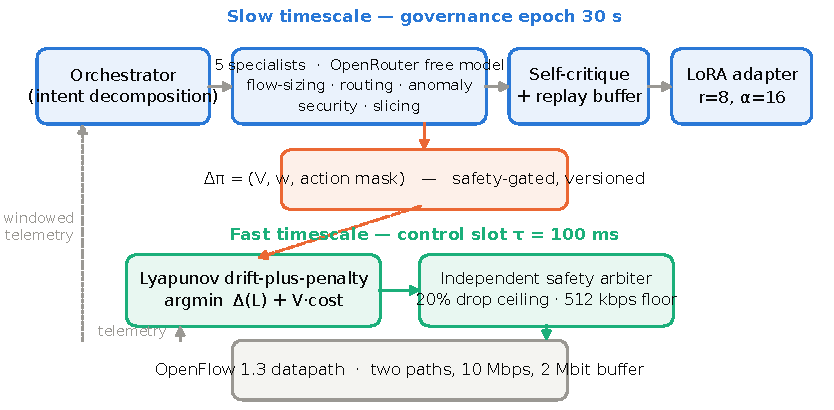
\includegraphics[width=\columnwidth]{figures/fig1_architecture.pdf}
\caption{The three loops and the single channel between them. The language model
emits only $\dpi=(V,\wvec,\mathcal{M})$; the fast loop emits rules; the arbiter sits
between the fast loop and the datapath and can veto either.}
\label{fig:arch}
\end{figure}

\subsection{Fast loop --- every $\tau=\ResTauMs$~ms}
Algorithm~\ref{alg:fast} is \eqref{eq:dpp} plus the arbiter. It runs on local
state only and never blocks on anything remote, which is why it can run at slot
rate.

\begin{algorithm}[t]
\caption{Fast loop (one slot)}\label{alg:fast}
\begin{algorithmic}[1]
\Require backlogs $\Qvec(t)$, demands $m(t),e(t)$, policy $(V,\wvec,\mathcal{M})$
\State $a^{\star} \gets \arg\min_{a\in\mathcal{M}}\big[\sum_i Q_i(t)(\lambda_i(a)-C_i) + V c(a)\big]$
\If{$a^{\star}=\texttt{rate\_limit}$}
  \State $r \gets \min\!\big(0.9C_0-m(t),\,0.85\,e(t)\big)\cdot 1000$ \Comment{kbps, synthesised locally}
\EndIf
\State $(a,\textit{veto}) \gets \textsc{SafetyArbiter}(a^{\star},r,\text{telemetry})$
\State install $a$; advance datapath by \eqref{eq:raw}--\eqref{eq:served}
\State \Return realised $(\rho,d,\ell)$ and the updated backlogs
\end{algorithmic}
\end{algorithm}

\subsection{Mid loop --- every $T_w=\ResWindowSec$~s}
A LoRA-adapted policy head proposes the action for the coming window. The base is a
pinned SmolLM2-135M-Instruct checkpoint~\cite{allal2025smollm2}, frozen, with a rank-8
$\alpha{=}16$ adapter on the \texttt{q\_proj} and \texttt{v\_proj}
projections~\cite{hu2022lora}. Decoding is constrained to three action tokens, and
\emph{no} numeric parameter is ever produced by the model: a chosen
\texttt{rate\_limit} is turned into a concrete meter rate by the same local
arithmetic the fast loop uses. The head answers in \ResThreeCtrl~ms on CPU, which is
what makes window-rate operation affordable.

The adapter is fitted on the replay buffer that stage~S2 accumulated while
controlling this same datapath, which is what ``experience internalised into
weights'' has to mean if the stage is to be an honest increment over the one
before it. Labels are advantage-filtered: for each quantised state the preferred
action is the one with the highest mean realised reward over that state's
immediate neighbourhood, with the exact state weighted double, and a state where
no neighbour ever tried a different action is kept only if its single action beat
the global mean reward. Training and gate seeds are disjoint, so the gate cannot
be passed by memorising a trajectory. The candidate is promoted only if its
agreement with the preferred action on held-out gate states exceeds the frozen
base by a declared margin; on this run it did, improving agreement from
\ResAdapterBase\ to \ResAdapterCandidate\ against a required margin of
\ResAdapterMargin. The loader refuses any adapter that cannot prove, through
parameter hashes recorded before and after the fit, that the base stayed frozen
and that the adapter weights actually moved.

\subsection{Slow loop --- every $T_g=\ResEpochSec$~s}
An orchestrator plus five specialists (flow sizing, routing, anomaly, security,
slicing) run as one panel request to a free-tier endpoint and return a merged
$\dpi=(\Delta V,\Delta\wvec,\mathcal{M})$. The deltas are clipped to
$|\Delta V|\le4$ and $|\Delta w_k|\le0.15$, the weights are renormalised, and the
mask may only shrink the admissible set. Stage S2 adds a second pass in which the
agent criticises its own proposal against the realised reward of the previous
window and a bounded episodic replay buffer, in the spirit
of~\cite{shinn2023reflexion,araujo2024agentic}. Algorithm~\ref{alg:slow} states the
epoch in full, including the two places it refuses its own model.

\begin{algorithm}[t]
\caption{Slow loop (one governance epoch)}\label{alg:slow}
\begin{algorithmic}[1]
\Require windowed telemetry $z$, current policy $(V,\wvec,\mathcal{M})$, replay buffer $\mathcal{B}$
\State $\rho \gets \textsc{PanelRequest}(z)$ \Comment{one request; orchestrator $+$ 5 specialists}
\If{$\rho$ is unusable or no endpoint answered}
  \State \Return $(V,\wvec,\mathcal{M})$ unchanged \Comment{declared fallback, counted}
\EndIf
\State $\Delta V \gets \mathrm{clip}(\rho.\Delta V, -4, 4)$
\State $\Delta w_k \gets \mathrm{clip}(\rho.\Delta w_k, -0.15, 0.15)$ for each $k$
\State $V \gets \mathrm{clip}(V + \Delta V,\ 0.5,\ 32)$
\State $\wvec \gets (\wvec + \Delta\wvec) / \lVert \wvec + \Delta\wvec \rVert_1$
\State $\mathcal{M} \gets \mathcal{A}$ \Comment{reset: a mask is scoped to one epoch only}
\If{$|\rho.\mathcal{M}| \ge 2$ \textbf{and} $\texttt{no\_op} \in \rho.\mathcal{M}$}
  \State $\mathcal{M} \gets \rho.\mathcal{M}$
\Else
  \State record \emph{mask rejected}: fewer than two admissible actions
\EndIf
\State append $(z, a, R)$ of the elapsed epoch to $\mathcal{B}$
\State \Return $(V,\wvec,\mathcal{M})$ to the fast loop
\end{algorithmic}
\end{algorithm}

Two properties of Algorithm~\ref{alg:slow} matter more than the rest. Line~9 resets
the mask before applying the proposal, so a single bad epoch cannot latch the
datapath into \texttt{no\_op} for the remainder of the run --- an earlier version
without that line did exactly that, and produced stage results byte-identical to
the static baseline. Lines~2--4 make the absence of a model answer an explicit,
counted outcome rather than a silent default.

\subsection{Safety arbiter}
The arbiter is ordinary deterministic code, outside both learned components. It
rejects a meter below 512 kbps, a meter discarding more than 20\% of the measured
flow rate, and a reroute that would push the destination link past 90\% of
capacity. A rejected proposal becomes \texttt{no\_op} and is counted: the paper
reports veto counts rather than hiding them.

\subsection{Charging the control plane for its own latency}\label{sec:lag}
This is the detail that makes the comparison fair. A proposal that takes $L$
seconds to produce cannot take effect at the start of the window it was computed
for. We therefore hold the previously installed rule for the first
$\lceil L/\tau\rceil$ slots of the window and apply the new one only afterwards. A
controller that thinks slowly is thus penalised exactly where it should be --- in
the datapath --- rather than only in a side table. The fast loop, acting on local
state within the slot, incurs no such lag.

$L$ here is the \emph{end-to-end} wait the slow loop experiences, not the HTTP
exchange alone: it includes the walk past endpoints that have exhausted their
daily allowance and the inter-request gap needed to stay inside a provider's
per-minute limit. That is the right quantity to charge, because the rule cannot
be installed until the answer arrives and the answer cannot arrive sooner without
breaking the provider's terms. A deployment with a funded key would pace less
aggressively and see a smaller $L$; the endpoint latency it would still pay is
the separate figure reported in Section~\ref{sec:serving}.

% =====================================================================
\section{Experimental Setup}\label{sec:setup}
% =====================================================================

\subsection{Configurations}
Six pipeline stages, each adding exactly one mechanism to the one before it:
S0 static forwarding; S1 a static LLM agent (zero-shot, no memory, no critique);
S2 $+$ self-critique and episodic replay; S3 $+$ the LoRA policy head;
S4 $+$ six-agent governance of $(V,\wvec,\mathcal{M})$; S5 $+$ the fast Lyapunov
loop. Three non-LLM controllers provide external reference points: a
capacity-aware threshold heuristic, a greedy least-loaded (ECMP-style) selector,
and a tabular $Q$-learner trained online on the same reward \eqref{eq:reward} and
the same action set.

\subsection{Protocol}
Every configuration is run on \ResSeeds~seeds (\ResSeedList), \ResWindows~windows of
\ResWindowSec~s each, i.e.\ \ResRunSec~s and \ResSlotsPerRun~slots per run, for
\ResTotalSlots~control slots in total. Within a seed all configurations see
bit-identical offered demand, so comparisons are paired at the (seed, window)
level. Traffic is produced by the frozen generator in \texttt{traffic\_gen.py} and
hashed into the result manifest.

All traffic is synthetic and seeded; nothing is captured or proprietary. Three
profiles are used: \texttt{steady\_bursty} for the main study (a steady mice
aggregate plus Poisson elephant bursts), \texttt{flash\_crowd} as the transfer
hold-out, and \texttt{volatile\_dpp} for the $V$ sweep. The stage-S3 adapter was
fitted for \ResAdapterSteps~optimiser steps over \ResAdapterTrainStates~training
states, updating \ResAdapterParams~LoRA parameters at rank \ResAdapterRank\ and
$\alpha=\ResAdapterAlpha$; its gate used \ResAdapterGateStates~states from seeds
excluded from training.

\subsection{Language-model serving}\label{sec:serving}
Decisions are served by free endpoints only; the client refuses any OpenRouter model
id without a \texttt{:free} suffix, so the study cannot incur billing. The primary
endpoint is \expandafter\nolinkurl\expandafter{\ResLLMModel}, with a \ResLLMChain-entry fallback chain spanning
two providers. The chain is not decoration: an unfunded OpenRouter key allows
50 free-model requests per day, and exhausting it mid-study is the normal case
rather than an edge case. Over the reported study \ResLLMDecisions~slow-loop
decisions were served, of which \ResLLMRequests~were live requests and
\ResLLMCached~were resolved from the recorded trace; \ResLLMFallbacks~decisions fell
back to the declared local default, giving a served fraction of \ResLLMServed\%.
One healthy request took \ResLLMLatency~ms on average
(95th percentile \ResLLMPNinetyFive~ms). That figure times the HTTP exchange
alone: the inter-request gap the client imposes to stay inside a provider's
per-minute limit is our own politeness and is deliberately excluded, because
charging it to the model would overstate exactly the quantity this paper is built
around. Including the walk past endpoints that had exhausted their daily
allowance, the mean wait rises to \ResLLMChainLatency~ms, and the circuit breaker
eventually tripped \ResLLMTripped\ of the \ResLLMChain\ chain entries.

We state plainly which endpoint produced the decisions this paper reports,
because it is not the configured primary. By the time the reported study ran, the
OpenRouter entries had exhausted their daily allowance and were tripped, and
\texttt{\ResLLMServedBy} answered \ResLLMServedByCount\ of the
\ResLLMDecisions~decisions (\ResLLMServedByPct\%). Nothing in the architecture
depends on that identity --- the decision interface is the same
$\dpi=(V,\wvec,\mathcal{M})$ whichever endpoint answers, and the safety arbiter is
downstream of all of them --- but a reader comparing latencies across papers is
entitled to know which model was on the other end of the connection.

\begin{figure}[t]
\centering
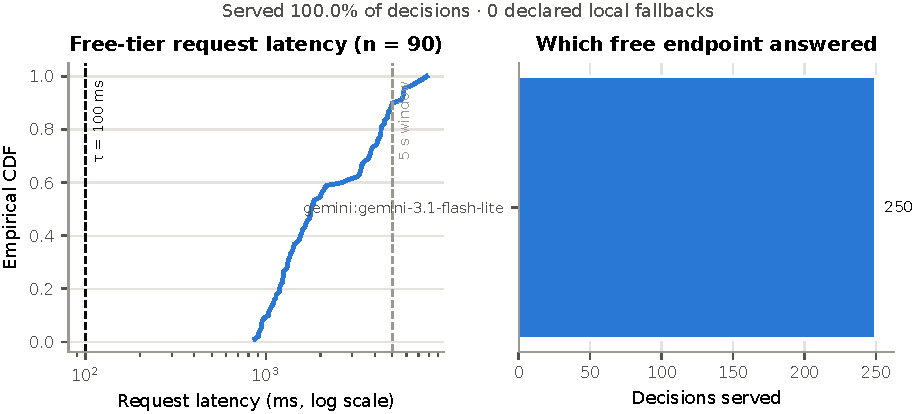
\includegraphics[width=\columnwidth]{figures/fig10_provider.pdf}
\caption{Free-tier serving behaviour: the latency distribution of a healthy
endpoint request, and which endpoint in the chain actually answered.}
\label{fig:provider}
\end{figure}

Figure~\ref{fig:provider} shows the resulting serving behaviour. Which endpoint
answers is not a fixed property of the configuration but of the daily allowance
remaining at the moment of the request, which is itself an argument for keeping
the model off the critical path.

\subsection{Reproducibility}\label{sec:reproducibility}
Every request is appended to a JSONL trace keyed by the SHA-256 of its role and
prompt, together with the endpoint that answered, the latency, and the token
counts. Re-running with \texttt{-{}-mode replay} resolves every decision from that
trace and requires no credential, reproducing every number in this paper exactly.
A third mode, \texttt{-{}-mode enumerate}, counts the prompts a live run would need
without spending quota, which is how the study was sized against the daily ceiling.
All figures and all numeric claims are regenerated from the result files by
\texttt{make\_paper\_macros.py} and \texttt{plot\_pipeline\_study.py}; no result is
typed into this manuscript by hand.

% =====================================================================
\section{Results}\label{sec:results}
% =====================================================================

\subsection{Offered load}
Figure~\ref{fig:traffic} shows one seed of the offered trace. Mean utilisation is
moderate, but superposed bursts push instantaneous demand above the 20~Mbps total
capacity in a minority of slots, which is the origin of the \ResFloorLoss\% floor
of \eqref{eq:floor}.

\begin{figure}[t]
\centering
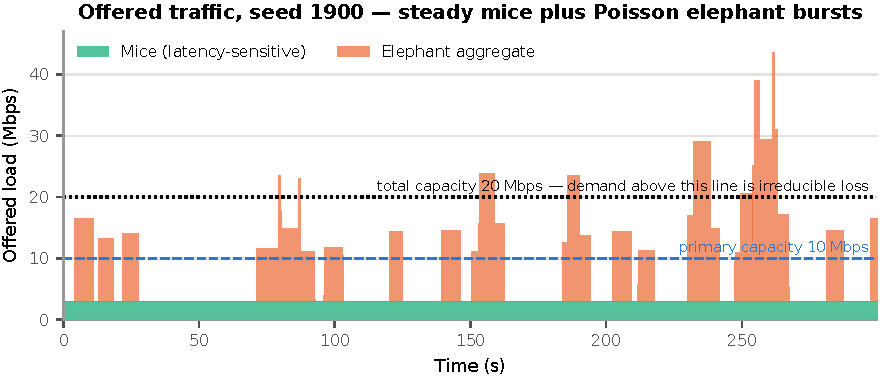
\includegraphics[width=\columnwidth]{figures/fig2_traffic.pdf}
\caption{Offered traffic for one seed.}
\label{fig:traffic}
\end{figure}

\subsection{Staged ablation}\label{sec:results-ablation}

\begin{table}[t]
\caption{Incremental pipeline ablation. Each stage adds one mechanism to the stage
above it. Mean over \ResSeeds\ paired seeds.}
\label{tab:ablation}
\centering
\footnotesize
\renewcommand{\arraystretch}{1.12}
\begin{tabular}{lrrrrrr}
\toprule
\textbf{Stage} & \textbf{Delay} & \textbf{P95} & \textbf{Tput} & \textbf{Loss} &
\textbf{$\bar{Q}$} & \textbf{Reward} \\
 & (ms) & (ms) & (Mbps) & (\%) & (Mbit) & \\
\midrule
\AblationRows
\bottomrule
\end{tabular}
\end{table}

Table~\ref{tab:ablation} and Fig.~\ref{fig:ablation} give the main result. Relative
to static forwarding, the full pipeline reduces mean delay by \ResLatVsStatic\%,
loss by \ResLossVsStatic\% and mean backlog by \ResQueueVsStatic\%. Relative to the
static LLM agent --- the configuration closest to~\cite{araujo2024agentic} --- the
reduction in delay is \ResLatVsLLM\%.

\begin{figure}[t]
\centering
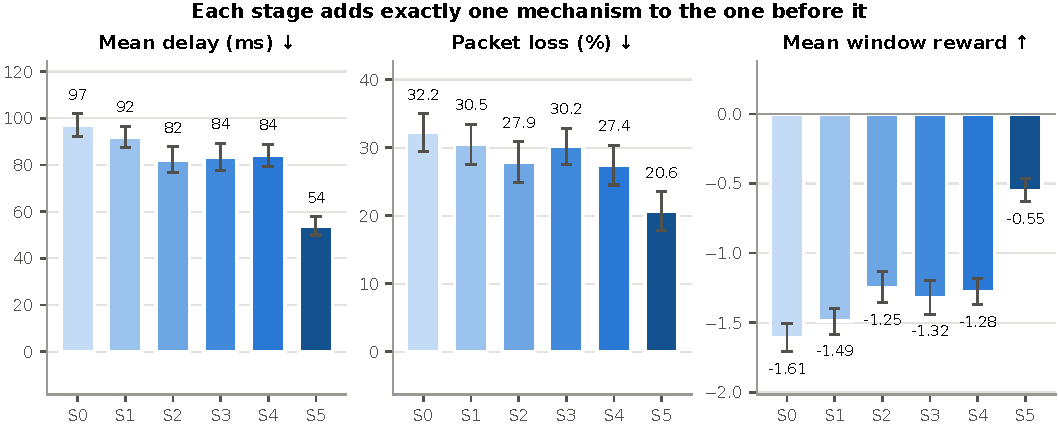
\includegraphics[width=\columnwidth]{figures/fig3_ablation.pdf}
\caption{Staged ablation; error bars are the standard error over seeds.}
\label{fig:ablation}
\end{figure}

\begin{figure}[t]
\centering
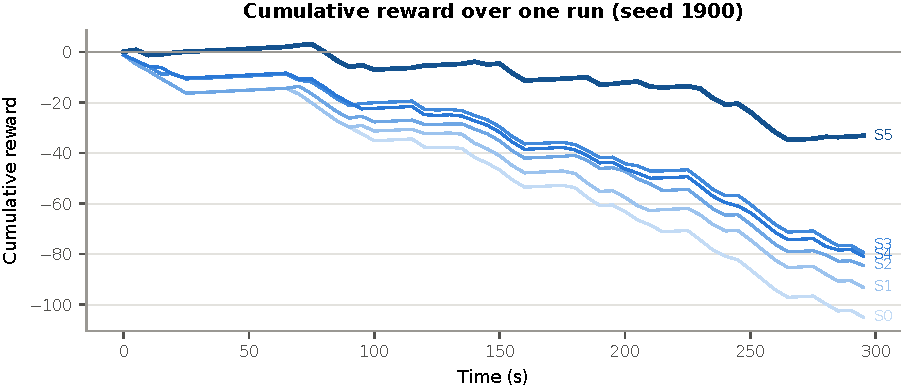
\includegraphics[width=\columnwidth]{figures/fig9_convergence.pdf}
\caption{Cumulative reward over one run. The separation opens within the first
governance epochs and widens monotonically; no stage needs a training phase
before it is useful, which is the practical difference from a value-based
learner.}
\label{fig:convergence}
\end{figure}

Figure~\ref{fig:convergence} shows cumulative reward over a single run. The
ordering is established early --- there is no exploration phase to pay for,
because the only learned component is fitted offline on replayed experience and
the fast loop is analytic.

\subsection{Why the model cannot sit in the fast loop}\label{sec:results-latency}

\begin{figure}[t]
\centering
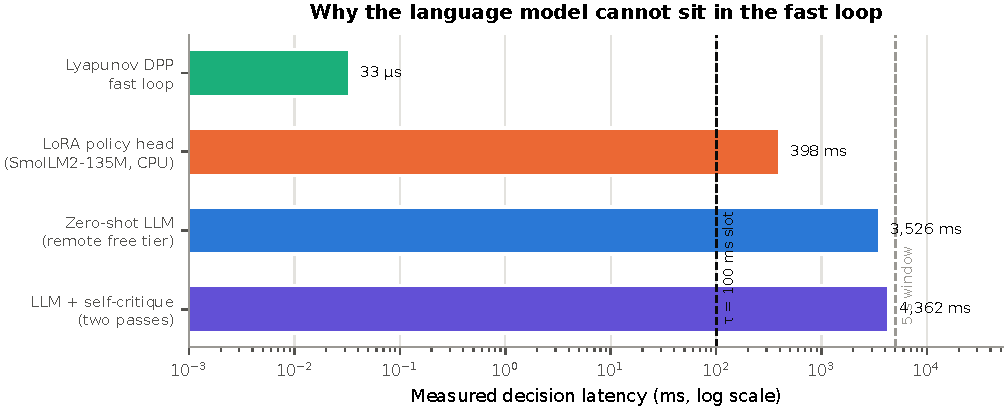
\includegraphics[width=\columnwidth]{figures/fig4_control_latency.pdf}
\caption{Measured decision latency against the two control periods, log scale.}
\label{fig:ctrl}
\end{figure}

Figure~\ref{fig:ctrl} is the quantitative core of the paper's argument. The slow
loop waits \ResOneCtrl~ms per decision in stage S1 and \ResTwoCtrl~ms in stage S2,
which issues two passes. Of that, \ResLLMLatency~ms is one healthy endpoint
request; the remainder is the chain walk past endpoints that have exhausted their
daily allowance (mean chain latency \ResLLMChainLatency~ms over the study, with
\ResLLMTripped\ of the \ResLLMChain\ chain entries eventually tripped). The local
LoRA head costs \ResThreeCtrl~ms and the drift-plus-penalty optimiser costs
\ResFastUs~\textmu s, roughly \ResSpeedup\,$\times$ faster than one remote
request. Against a \ResTauMs~ms slot, only the last of these
is admissible at slot rate, and only the LoRA head is admissible at window rate.
The three-timescale decomposition is not a design preference; it is what these
three numbers permit.

\subsection{Loss accounting}\label{sec:results-loss}

\begin{figure}[t]
\centering
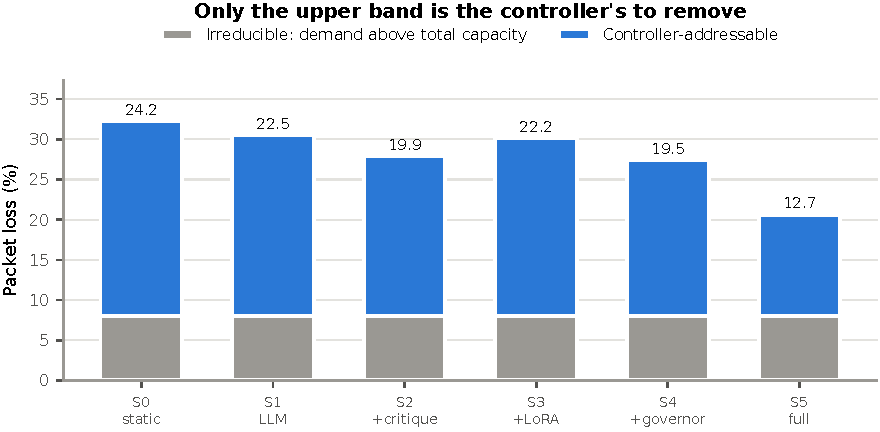
\includegraphics[width=\columnwidth]{figures/fig8_loss_decomposition.pdf}
\caption{Measured loss split into the floor imposed by demand above total capacity
and the controller-addressable remainder.}
\label{fig:lossdecomp}
\end{figure}

Figure~\ref{fig:lossdecomp} separates the two. Of the \ResZeroLoss\% loss under
static forwarding, \ResFloorLoss\ percentage points are structurally unavoidable;
the full pipeline removes a substantial part of the remainder, taking addressable
loss from \ResZeroExcess\% to \ResFiveExcess\%. Reporting the total alone would
have overstated what the controller achieves.

\subsection{Queue stability and the $V$ knob}

\begin{figure}[t]
\centering
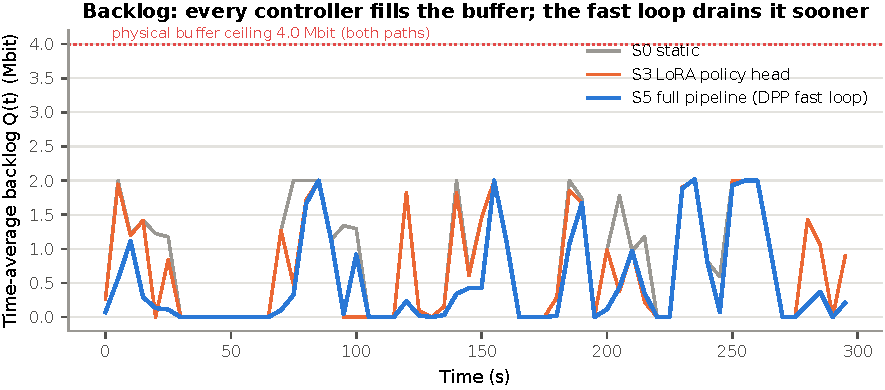
\includegraphics[width=\columnwidth]{figures/fig5_queue.pdf}
\caption{Backlog trajectory for one seed.}
\label{fig:queue}
\end{figure}

\begin{figure}[t]
\centering
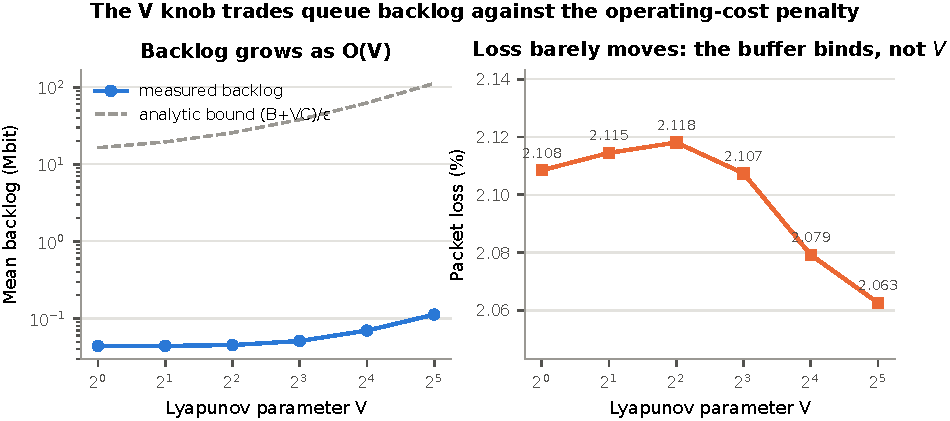
\includegraphics[width=\columnwidth]{figures/fig6_v_tradeoff.pdf}
\caption{Sweeping $V$ over $[\ResVMin,\ResVMax]$ on the volatile profile.}
\label{fig:vtradeoff}
\end{figure}

Figure~\ref{fig:queue} shows backlog over time. Figure~\ref{fig:vtradeoff} sweeps
$V$ on a dedicated high-volatility profile: mean backlog rises from
\ResVBacklogMin~Mbit at $V{=}\ResVMin$ to \ResVBacklogMax~Mbit at $V{=}\ResVMax$,
the $O(V)$ growth Theorem~\ref{thm:bound} predicts, and measured backlog stays
below the analytic ceiling \eqref{eq:bound} at \ResVCompliance\% of the swept
operating points.

The matching $O(1/V)$ fall in the penalty term is present but negligible here:
loss moves only from \ResVLossMin\% to \ResVLossMax\% across a 32-fold change in
$V$, and not monotonically at the small-$V$ end. We report that rather than
presenting the panel as a clean confirmation, because the reason is informative.
In this regime the 2~Mbit physical buffer binds long before either the analytic
ceiling or the penalty weight does, so $V$ has little room to trade anything
away. The same fact makes the bound loose: its satisfaction is a consistency
check on the derivation, not evidence that it is tight. A deeper buffer, or an
offered load closer to the capacity region's edge, would be needed to exercise
the trade-off properly.

\subsection{Comparison against non-LLM controllers}

\begin{table}[t]
\caption{Comparison on the identical trace. Control latency is the measured
per-decision cost of the control plane.}
\label{tab:baselines}
\centering
\footnotesize
\renewcommand{\arraystretch}{1.12}
\setlength{\tabcolsep}{3pt}
\begin{tabular}{@{}>{\raggedright\arraybackslash}p{0.35\columnwidth}rrrrr@{}}
\toprule
\textbf{Controller} & \textbf{Delay} & \textbf{P95} & \textbf{Loss} &
\textbf{Reward} & \textbf{Ctrl} \\
 & (ms) & (ms) & (\%) & & (ms) \\
\midrule
\BaselineRows
\bottomrule
\end{tabular}
\end{table}

\begin{figure}[t]
\centering
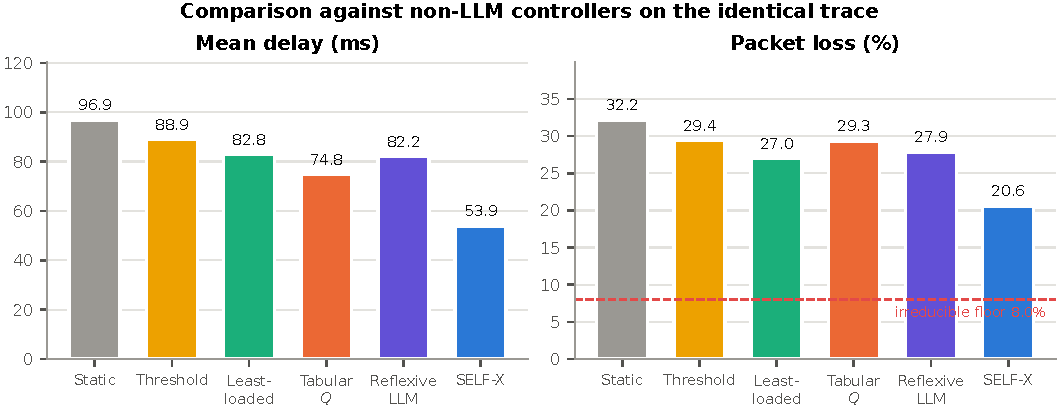
\includegraphics[width=\columnwidth]{figures/fig7_baselines.pdf}
\caption{Delay and loss against non-LLM controllers.}
\label{fig:baselines}
\end{figure}

Table~\ref{tab:baselines} and Fig.~\ref{fig:baselines} place the pipeline against
the external references. The tabular $Q$-learner is the strongest non-LLM
comparator and still trails the full pipeline by \ResLatVsQ\% in delay, while paying
the cold-start cost the learned-controller literature
describes~\cite{xu2018experience,boussaoud2025marl}.

\subsection{Statistical significance}

\begin{table}[t]
\caption{Paired window-level tests against the full pipeline. $n$ is the number of
matched (seed, window) pairs; the interval is a seed-level cluster bootstrap.}
\label{tab:stats}
\centering
\footnotesize
\renewcommand{\arraystretch}{1.12}
\begin{tabular}{lrrrr}
\toprule
\textbf{Comparison} & \textbf{$n$} & \textbf{$t$} & \textbf{$p$} & \textbf{Cohen's $d$} \\
\midrule
S5 vs.\ S0 & \StatSFivevsSZeroN & \StatSFivevsSZeroT & \StatSFivevsSZeroP & \StatSFivevsSZeroD \\
S5 vs.\ S1 & \StatSFivevsSOneN  & \StatSFivevsSOneT  & \StatSFivevsSOneP  & \StatSFivevsSOneD \\
S5 vs.\ S2 & \StatSFivevsSTwoN  & \StatSFivevsSTwoT  & \StatSFivevsSTwoP  & \StatSFivevsSTwoD \\
S5 vs.\ S4 & \StatSFivevsSFourN & \StatSFivevsSFourT & \StatSFivevsSFourP & \StatSFivevsSFourD \\
S5 vs.\ $Q$& \StatSFivevsQN     & \StatSFivevsQT     & \StatSFivevsQP     & \StatSFivevsQD \\
\bottomrule
\end{tabular}
\end{table}

Pairing on matched windows rather than on seeds raises $n$ from \ResSeeds\ to
\StatSFivevsSZeroN\ while keeping the comparison matched. Because windows inside a
seed are serially dependent, Table~\ref{tab:stats} reports the paired $t$ statistic
alongside a seed-level cluster bootstrap, and the bootstrap interval is what we rely
on. The family-wise threshold after Bonferroni correction is
$\alpha=\StatBonferroni$.

\subsection{Zero-shot transfer}
Freezing the policy produced on the training profile and evaluating it, without any
adaptation, on the held-out \ResTransferProfile\ profile retains
\ResTransferRetention\% of its reward gain over that profile's own static baseline
(train gain \ResTransferTrainGain, held-out gain \ResTransferHoldGain). Measuring
against the held-out profile's own baseline matters: a harder workload would
otherwise inflate retention.

This is a partial result and we report it as one. Roughly a quarter of the gain
does not survive the shift, which is unsurprising given what the two profiles are:
the training profile has Poisson-arriving bursts separated by quiet intervals, and
the held-out profile sustains a three-fold flash crowd through its middle third,
so the backlog regime the controller spends most of its time in is different. The
transferable part is the fast loop, whose decision rule is analytic and carries no
fitted parameters; what does not transfer is the $(V,\wvec)$ operating point the
governor settled on for the training workload. That points at an obvious next
step --- let the governance epoch re-tune on the new profile, which is exactly the
mechanism it exists for --- but we have not run it, so we do not claim it.

% =====================================================================
\section{Discussion and Limitations}\label{sec:discussion}
% =====================================================================

\textbf{What the ablation does not show.} The stages are not uniformly monotone.
Adding multi-agent governance (S4) does not improve every metric over the LoRA
stage (S3): the governor spends part of each epoch exploring the $(V,\wvec)$ space,
and that exploration costs reward in the windows where it narrows the action mask
unnecessarily. The improvement at S5 comes predominantly from the fast loop, not
from the governance layer, and Table~\ref{tab:ablation} should be read that way. We
report this because an ablation in which every stage happens to help is usually an
ablation that has been tuned until it does.

\textbf{The datapath is a fluid model, not hardware.} Results come from a
bit-conserving finite-buffer fluid simulation of a two-path OpenFlow topology, not
from a Mininet or hardware testbed. The model's conservation and queue integrals
are exact and asserted on every slot, but it abstracts away TCP dynamics, per-packet
scheduling, control-channel contention and real flow-mod installation times. Claims
about \emph{relative} ordering of controllers on this datapath are well supported;
absolute millisecond values are model outputs and should not be read as hardware
measurements.

\textbf{Free-tier serving is a real constraint, not an artefact.} With a 50-request
daily ceiling and \ResLLMFallbacks\ declared fallbacks, any deployment resembling
this one must be fail-operational by construction. We treat that as a finding: a
language-model control plane needs a declared local default and an accounting of how
often it is used, which is precisely what the served-fraction metric reports.

\textbf{The adapter gate is thin.} The replay buffer stage~S2 produced collapses
to \ResAdapterStates\ distinct quantised states, of which \ResAdapterTrainStates\
train the adapter and \ResAdapterGateStates\ hold it out. An eleven-state gate can
detect a clearly better or clearly worse candidate, which is what it is for, but
it cannot resolve small differences, and a promotion decision taken on it should
be read as a sanity check rather than as a model-selection result. A longer run,
or several runs pooled, would give the gate more to work with; we report the
number of states rather than only the agreement figure so the reader can weigh
the decision accordingly.

\textbf{Generalisation is partial.} The frozen policy retains
\ResTransferRetention\% of its gain on the held-out profile, below the 90\% we set
as a target before running it. We report the measured number, not the target. The
analytic fast loop transfers because it has no fitted parameters; the
governance-chosen $(V,\wvec)$ operating point does not.

\textbf{Scope.} One topology family, one workload generator with three profiles, and
one small adapter base. Generalisation across topologies is evidenced only by the
single held-out profile of Section~\ref{sec:results} and should be treated as
indicative.

% =====================================================================
\section{Conclusion}
% =====================================================================

SELF-X separates software-defined flow control into three loops whose periods are
set by the measured cost of the mechanism running in each: an analytic Lyapunov
optimiser at \ResTauMs~ms carrying a provable backlog bound, a LoRA-adapted policy
head at \ResWindowSec~s, and a multi-agent language-model governor at
\ResEpochSec~s that emits only a safety-gated $(V,\wvec,\mathcal{M})$ delta. Against
static forwarding the full pipeline reduces delay by \ResLatVsStatic\% and loss by
\ResLossVsStatic\%, and the strictly incremental ablation attributes those gains to
specific mechanisms rather than to the architecture as a whole. The negative result
matters as much as the positive one: the governance layer is not where most of the
gain comes from, and a remote model is roughly \ResSpeedup\,$\times$ slower than
the loop that has to react --- which is exactly why it belongs on the slowest
loop, setting the objective rather than installing the rules.

The obvious next step is to replace the fluid datapath with Mininet and Open
vSwitch and re-run this identical harness against a real control channel, which
would turn the actuation-lag model of Section~\ref{sec:lag} from an assumption
into a measurement. Two smaller ones follow from the results rather than from
ambition: letting the governance epoch re-tune $(V,\wvec)$ on a shifted workload,
which is the mechanism the transfer shortfall points at, and pooling several runs
so the adapter's promotion gate has more than eleven held-out states to judge on.

\section*{Author Contributions}
Ganesh Reddy J designed the agent architecture, the LoRA policy head and the
weight-adaptation pipeline. M Jagadeswar built the evaluation harness, the
result-persistence layer and the data-integrity checks. Harsh Raj built the
dashboard, the figure pipeline and this manuscript. C Sai Aravind derived and
validated the drift-plus-penalty formulation and the backlog bound. Koushik C
built the free-tier provider client, its record-and-replay contract and the
reproducibility tooling. Dhruv R Katti built the traffic generator, the datapath
model and its conservation checks. All six authors designed the study and
reviewed the analysis.

\section*{Acknowledgment}
The authors thank Prof.\ Jagadeesha R.\ Bhat, Assistant Professor, Department of
Data Science and Artificial Intelligence, IIIT Dharwad, for supervising this work
and in particular for the question that reshaped it: what, precisely, does this
architecture contribute beyond the sum of the systems it borrows from? Section~II
is the answer, and the staged ablation of Section~VII is the evidence for it.

\section*{Artefact Availability}
Source, frozen traffic traces, the recorded language-model trace, the result files
and the scripts that regenerate every figure and every number in this paper are
included in the submission archive. \texttt{scripts/run\_all.ps1 -Replay}
reproduces the complete study from the recorded trace without any credential.

\bibliographystyle{IEEEtran}
\bibliography{refs}

\end{document}
